\documentclass[10pt,a4paper]{article}

\usepackage[utf8]{inputenc}
\usepackage[T1]{fontenc}
\usepackage{lmodern}
\usepackage[ngerman]{babel}
\usepackage[margin=1.5cm,top=1.3cm,bottom=1.6cm]{geometry}
\usepackage{amsmath,amssymb}
\usepackage{booktabs}
\usepackage{graphicx}
\usepackage{listings}
\usepackage[dvipsnames]{xcolor}
\usepackage[most]{tcolorbox}
\usepackage{enumitem}
\usepackage{titlesec}
\usepackage[hidelinks,pdftitle={Assignment 2 - Spickzettel},pdfauthor={},pdfcreator={},pdfproducer={}]{hyperref}
\pdfstringdefDisableCommands{\def\code#1{#1}}

\graphicspath{{../plotting/}}

\setlength{\parindent}{0pt}
\setlength{\parskip}{3pt}
\setlength{\emergencystretch}{2em}
\setlist{nosep,leftmargin=1.3em}

\definecolor{blau}{HTML}{2A78D6}
\definecolor{orange}{HTML}{EB6834}
\definecolor{grau}{HTML}{F3F5F8}

\titleformat{\section}{\Large\bfseries\color{blau}}{}{0pt}{}[\vspace{-2pt}{\color{blau}\titlerule[0.8pt]}]
\titleformat{\subsection}{\large\bfseries}{}{0pt}{}
\titlespacing*{\section}{0pt}{9pt}{4pt}
\titlespacing*{\subsection}{0pt}{8pt}{3pt}
\makeatletter
\newcommand{\secneed}[1]{\par\penalty\@M\begingroup\setlength{\dimen@}{#1}\dimen@ii\pagegoal
  \advance\dimen@ii-\pagetotal\ifdim\dimen@>\dimen@ii\ifdim\dimen@ii>\z@\vfil\fi\penalty-\@M\fi\endgroup}
\makeatother
\let\oldsection\section
\renewcommand{\section}{\secneed{9\baselineskip}\oldsection}

\lstset{
  language=C++,
  basicstyle=\ttfamily\footnotesize,
  keywordstyle=\color{blau}\bfseries,
  commentstyle=\color{gray}\itshape,
  numbers=left,
  numberstyle=\tiny\color{gray},
  numbersep=6pt,
  backgroundcolor=\color{grau},
  frame=leftline,
  rulecolor=\color{blau},
  framerule=2pt,
  xleftmargin=18pt,
  columns=fullflexible,
  keepspaces=true,
  showstringspaces=false,
  aboveskip=4pt,
  belowskip=2pt,
  literate={ä}{{\"a}}1 {ö}{{\"o}}1 {ü}{{\"u}}1
}

\newtcolorbox{fragen}{
  enhanced, breakable, colback=orange!6, colframe=orange, boxrule=0.6pt, arc=2pt,
  left=6pt, right=6pt, top=4pt, bottom=4pt,
  title={\bfseries Mögliche Fragen}, coltitle=white, fonttitle=\bfseries, fontupper=\small
}
\newtcolorbox{merke}{
  enhanced, colback=blau!6, colframe=blau, boxrule=0.6pt, arc=2pt,
  left=6pt, right=6pt, top=4pt, bottom=4pt
}
\newtcolorbox{herleitung}[1]{
  enhanced, breakable, colback=blau!6, colframe=blau, boxrule=0.6pt, arc=2pt,
  left=6pt, right=6pt, top=4pt, bottom=4pt,
  title={\bfseries Herleitung: #1}, coltitle=white, fonttitle=\bfseries
}
\newtcolorbox{extra}{
  enhanced, breakable, colback=gray!7, colframe=gray!70!black, boxrule=0.6pt, arc=2pt,
  left=6pt, right=6pt, top=4pt, bottom=4pt,
  title={\bfseries Nur falls nachgefragt -- steht so nicht im Bericht (eigene Rechnung)},
  coltitle=white, fonttitle=\bfseries, fontupper=\small
}

\tcbset{before skip=5pt, after skip=5pt}

\newcommand{\frage}[2]{\textbf{F: #1}\par\nopagebreak\vspace{1pt}\textbf{A:} #2\par\vspace{5pt}}
\newcommand{\sagen}[1]{\textbf{Kurz gesagt:} \emph{#1}\par}
\newcommand{\code}[1]{\texttt{#1}}

\begin{document}
\small

{\LARGE\bfseries Assignment 2 -- Spickzettel für die Präsentation}\par
\vspace{2pt}
{\large Code aus \code{forwardkinematics.cpp} und \code{control.cpp}, Gains aus \code{gains\_1.txt},
Zahlen aus dem Bericht}

%=====================================================================
\section{Auf einen Blick}
%=====================================================================

{\small\setlength{\tabcolsep}{4pt}
\begin{tabular}{@{}llll@{}}
  \toprule
  Task & Funktion & Was passiert & Ergebnis \\
  \midrule
  A1 & \code{computeDH} & DH-Tabelle (Craig) & $\theta_2 = q_2 - \frac{\pi}{2}$, sonst nur $L_1, L_2, L_3$ \\
  A2 & \code{computeT0\_1} \ldots{} \code{computeT0\_E} & Transformationen & ${}^0_ET$ vereinfacht, $(x, y)$ bei $q = 0$: $(0.41, -0.49)$ \\
  A3 & \code{computeF} & $F = (x, y, \alpha)$ & $\alpha = q_1 + q_2 + q_3 - \frac{\pi}{2}$, bei $q = 0$: $\alpha = -1.57$ \\
  A4 & \code{computeJ} & $J = \partial F / \partial q$ & letzte Zeile $(1, 1, 1)$ \\
  A5 & Skizze & Spalten von $J$ als Pfeile & i steuerbar, ii nahe, iii in Singularität \\
  B1 & Rechnung & 2 kubische Splines + Via & $\dot q_b = (-0.31,\ 0,\ 0)$\,rad/s \\
  B2 & \code{computeTf}, \code{computeSpline}, \code{followSpline} & Spline + PD + $G$ & proj1: $t_f = 2.46$\,s, Fehler $< 0.01$\,rad \\
  C1 & \code{setCircleTarget}, \code{proj2Control} & Kreis, $\beta = \dot\beta\,t$ & 5\,s pro Runde, $0.25$\,m/s \\
  C2 & \code{operationalSpaceControl} & $\tau = J^T F + G$ & keine inverse Kinematik \\
  C3 & Gains & Fehler $\sim 1/k_p$ & max.\ 11\,mm, RMS 7\,mm, $\tau_1$ bis 116\,Nm \\
  C4 & \code{proj3Control} & Parabolic Blends für $\beta$ & $t_b = 5$\,s, $t_f = 20$\,s, $\tau_1$ bis 68\,Nm \\
  C5 & \code{line}, \code{xtrack}, \code{nxtrack}, \code{ntrack} & Bonus & max.\ Kreis 11, Linie 22, Quadrat 50\,mm \\
  \bottomrule
\end{tabular}
}

\subsection{Gains und Zahlen}
{\small
\begin{tabular}{@{}lll@{}}
  \toprule
  Regler (Nummer in \code{kp}/\code{kv}-Befehl) & $k_p$ & $k_v$ \\
  \midrule
  \code{njtrack} (11), \code{proj1} (21) & $3000 / 1350 / 300$ (Gelenke) & $245 / 70 / 21$ \\
  \code{proj2} (22), \code{proj3} (23) & $8000 / 8000 / 200$ ($x, y, \alpha$) & $280 / 280 / 10$ \\
  Bonus: \code{nxtrack} (13), \code{xtrack} (14), \code{ntrack} (17), \code{line} (20) & wie \code{proj2} & wie \code{proj2} \\
  \bottomrule
\end{tabular}
}

\begin{itemize}
  \item $L_1 = 0.41$\,m, $L_2 = 0.43$\,m, $L_3 = 0.055$\,m (\code{l1}, \code{l2}, \code{l3} im Header). Abkürzungen wie im
        Bericht: $s_1 = \sin q_1$, $c_{12} = \cos(q_1 + q_2)$, $s_{123} = \sin(q_1 + q_2 + q_3)$ usw.
  \item Simulator: $\dot q_{\max} = 0.79$\,rad/s, $\ddot q_{\max} = 1.05$\,rad/s$^2$ für alle Gelenke,
        $\tau_{\max} = 156.4 / 89.4 / 20.1$\,Nm.
\end{itemize}

\subsection{Zwei Koordinatensysteme}
\begin{minipage}[t]{0.49\textwidth}
\textbf{Fig.~1 (Teil A, \code{forwardkinematics.cpp})}
\begin{itemize}
  \item $x_0$ rechts, $y_0$ \textbf{nach unten}, $z_0$ in die Seite hinein.
  \item Positive Winkel = \textbf{im Uhrzeigersinn} im Bild.
  \item Nullstellung: Glied 1 waagerecht nach rechts, Glied 2 und 3 senkrecht nach oben.
  \item Hand oben $\Rightarrow$ $y < 0$ und $\alpha = -\frac{\pi}{2}$.
\end{itemize}
\end{minipage}\hfill
\begin{minipage}[t]{0.49\textwidth}
\textbf{Simulator (Teil C, \code{gv.x})}
\begin{itemize}
  \item $x$ rechts, $y$ \textbf{nach oben}, $z$ aus dem Bildschirm heraus.
  \item $\alpha = 0$ heißt aufrecht. Das Blatt sagt: $y$ ist umgekehrt zu Fig.~1.
  \item In Teil C nehmen wir nur Werte des Simulators (\code{gv.x}, \code{gv.dx}, \code{gv.Jtranspose}, \code{gv.G}),
        also keine Umrechnung im Code.
\end{itemize}
\end{minipage}

\vspace{2pt}
(Beobachtung im Simulator: Bei $q = 0$ zeigt \code{gv.x} $= (0.41,\ 0.59,\ 0)$. $F$ aus Teil A und \code{gv.x} also nicht
direkt vergleichen, der Nullpunkt ist ein anderer.)

\subsection{Demo im Simulator (Konsole \code{CS225A:>})}
\begin{enumerate}
  \item 3-DOF-Modus: \code{robottype 1}. In der GUI \glqq torque limits\grqq{} aus und \glqq Load gains\grqq{}
        (\code{loadgains} geht in der Konsole nicht; dort z.\,B.\ \code{kp 21 3000 1350 300}, \code{kv 21 245 70 21}).
  \item \code{proj1 0 0 0} -- fährt in 2.46\,s zum Kreisstart $(0.8,\ 0.35)$, danach Float. Die drei Zahlen werden ignoriert,
        die Konsole will aber drei Argumente.
  \item \code{proj2} -- Kreis, 5\,s pro Runde, läuft weiter, bis ein anderer Regler startet. (Meldet die Konsole
        \glqq expected \ldots{} args\grqq, Nullen anhängen wie bei proj1.)
  \item \code{proj1 0 0 0}, dann \code{proj3} -- drei Runden in 20\,s, sanft an und aus, hält danach den Endpunkt.
  \item Bonus, jeweils nach \code{proj1 0 0 0}: \code{line 0 0 0}, \code{xtrack 0 0 0 0}, \code{nxtrack 0 0 0 0},
        \code{ntrack 0 0 0}.
  \item \code{njtrack}: Zielwinkel in der GUI eingeben und starten, der Arm fährt auf einem Spline dorthin.
\end{enumerate}
Die Konsole schafft nur etwa einen Befehl pro Sekunde, also langsam tippen.

%=====================================================================
\section{A1: DH-Parameter}
%=====================================================================

\begin{center}
\begin{tabular}{ccccc}
  \toprule
  $i$ & $\alpha_{i-1}$ & $a_{i-1}$ & $d_i$ & $\theta_i$ \\
  \midrule
  1    & 0 & 0     & 0 & $q_1$ \\
  2    & 0 & $L_1$ & 0 & $q_2 - \frac{\pi}{2}$ \\
  3    & 0 & $L_2$ & 0 & $q_3$ \\
  4(E) & 0 & $L_3$ & 0 & 0 \\
  \bottomrule
\end{tabular}
\end{center}
\vspace{-6pt}
\begin{itemize}
  \item $\boldsymbol{\alpha = 0}$: Der Arm ist eben, alle $z$-Achsen sind parallel. $\boldsymbol{d = 0}$: Alle Frames
        liegen in einer Ebene, keine Verschiebung entlang $z$.
  \item $\boldsymbol{a_{i-1}}$: Abstand der Gelenkachsen = Gliedlänge. $a_0 = 0$, weil Frame 0 und 1 im selben Punkt liegen.
  \item $\boldsymbol{\theta_i}$: alle Gelenke drehen, also $q_i$ in $\theta_i$. $\theta_4 = 0$: zwischen Frame 3 und E
        ist kein Gelenk.
\end{itemize}

\textbf{Theorie in zwei Sätzen (Tutorial, Craig):} Die DH-Konvention beschreibt die Transformation zwischen zwei Frames
mit nur vier Zahlen. $\alpha_{i-1}$ und $a_{i-1}$ gehören zur $x$-Achse (Winkel und Abstand zwischen zwei $z$-Achsen),
$d_i$ und $\theta_i$ zur $z$-Achse (Abstand und Winkel zwischen zwei $x$-Achsen); bei einem Drehgelenk steckt $q_i$ in
$\theta_i$.

\textbf{Das $-\frac{\pi}{2}$ in Zeile 2:} $\theta_2$ ist der Winkel von $x_1$ nach $x_2$ um $z_2$. In der Nullstellung zeigt
$x_1$ nach rechts, $x_2$ aber nach oben. Die Frames sind also schon bei $q_2 = 0$ gegeneinander verdreht. $z$ zeigt in die
Seite hinein, positive Winkel gehen im Uhrzeigersinn. Von \glqq rechts\grqq{} nach \glqq oben\grqq{} ist gegen den
Uhrzeigersinn, also $-\frac{\pi}{2}$. Zwischen $x_2$ und $x_3$ (beide oben) gibt es keinen Versatz.

\secneed{2\baselineskip}
\begin{lstlisting}[firstnumber=112]
const float HALF_PI = 1.57079633f;
\end{lstlisting}
\vspace{-4pt}
\secneed{6\baselineskip}
\begin{lstlisting}[firstnumber=418]
   //row vector: frame 2
   DH[1][0] = 0.0;
   DH[1][1] = l1;
   DH[1][2] = 0.0;
   DH[1][3] = angles[1] - HALF_PI;
\end{lstlisting}
\textbf{Z.\,112, 410--435:} Jede Zeile von \code{DH} ist eine Zeile der Tabelle, in der Reihenfolge
$(\alpha_{i-1}, a_{i-1}, d_i, \theta_i)$. \code{HALF\_PI} ist eine eigene Konstante, weil wir keine weiteren Includes
benutzen dürfen.

\sagen{Alle Achsen sind parallel, deshalb ist $\alpha$ und $d$ überall null. Es bleiben die Gliedlängen in $a$ und die
Gelenkwinkel in $\theta$, plus ein fester Versatz von $-\frac{\pi}{2}$ an Gelenk 2, weil Glied 1 waagerecht und Glied 2
senkrecht steht.}

\begin{fragen}
\frage{Warum $-\frac{\pi}{2}$ und nicht $+\frac{\pi}{2}$?}
{$y_0$ zeigt nach unten, $z$ also in die Seite hinein, und positive Winkel gehen im Uhrzeigersinn. Von $x_1$ (rechts)
nach $x_2$ (oben) dreht man gegen den Uhrzeigersinn, das ist negativ. Prüfen kann man es an $q = 0$: Dann kommt
$(0.41, -0.49)$ heraus, die Hand ist oben, wie in Fig.~1.}
\frage{Ist die DH-Tabelle eindeutig?}
{Allgemein nicht (Tutorial): Die Richtung von $z$ ist frei, bei parallelen Achsen ist der Ursprung entlang der Achse
frei, bei sich schneidenden Achsen gibt es zwei Richtungen für $x$. Hier legt Fig.~1 die Frames aber fest, und für diese
Frames ist die Tabelle eindeutig.}
\frage{Warum fällt Frame 0 mit Frame 1 zusammen?}
{So legt man Frame 0 nach der Konvention (Tutorial, Schritt 7): gleicher Ursprung, gleiche $z$-Achse. Dann sind
$\alpha_0 = a_0 = d_1 = 0$, also möglichst viele Nullen, und ${}^0_1T$ ist eine reine Drehung um $q_1$. In Fig.~1 steht
deshalb $x_{0,1}$, $y_{0,1}$.}
\end{fragen}

%=====================================================================
\section{A2: Transformationen und Vorwärtskinematik}
%=====================================================================

\textbf{Original (Tutorial, Craig S.~74)} und \textbf{vereinfacht} mit $\alpha_{i-1} = 0$, $d_i = 0$
($c\alpha = 1$, $s\alpha = 0$):
\[
  {}^{i-1}_{\;\;i}T =
  \begin{pmatrix}
    c\theta_i & -s\theta_i & 0 & a_{i-1} \\
    s\theta_i\, c\alpha_{i-1} & c\theta_i\, c\alpha_{i-1} & -s\alpha_{i-1} & -s\alpha_{i-1}\, d_i \\
    s\theta_i\, s\alpha_{i-1} & c\theta_i\, s\alpha_{i-1} & c\alpha_{i-1} & c\alpha_{i-1}\, d_i \\
    0 & 0 & 0 & 1
  \end{pmatrix}
  \;\Rightarrow\;
  \begin{pmatrix}
    c\theta_i & -s\theta_i & 0 & a_{i-1} \\
    s\theta_i & c\theta_i & 0 & 0 \\
    0 & 0 & 1 & 0 \\
    0 & 0 & 0 & 1
  \end{pmatrix}
\]
Also nur eine Drehung um $z$ um $\theta_i$ und eine Verschiebung um $a_{i-1}$ entlang $x$. Für Zeile 2 die
\textbf{Verschiebungs-Identitäten} $\cos(q_2 - \frac{\pi}{2}) = s_2$, $\sin(q_2 - \frac{\pi}{2}) = -c_2$:
\[
  {}^0_1T = \begin{pmatrix} c_1 & -s_1 & 0 & 0 \\ s_1 & c_1 & 0 & 0 \\ 0&0&1&0 \\ 0&0&0&1 \end{pmatrix}
  \quad
  {}^1_2T = \begin{pmatrix} s_2 & c_2 & 0 & L_1 \\ -c_2 & s_2 & 0 & 0 \\ 0&0&1&0 \\ 0&0&0&1 \end{pmatrix}
  \quad
  {}^2_3T = \begin{pmatrix} c_3 & -s_3 & 0 & L_2 \\ s_3 & c_3 & 0 & 0 \\ 0&0&1&0 \\ 0&0&0&1 \end{pmatrix}
  \quad
  {}^3_ET = \begin{pmatrix} 1 & 0 & 0 & L_3 \\ 0 & 1 & 0 & 0 \\ 0&0&1&0 \\ 0&0&0&1 \end{pmatrix}
\]
\textbf{Kette} ${}^0_ET = {}^0_1T\,{}^1_2T\,{}^2_3T\,{}^3_ET$, Schritt für Schritt multipliziert und mit den
\textbf{Additionstheoremen} $s_{12} = s_1 c_2 + c_1 s_2$, $c_{12} = c_1 c_2 - s_1 s_2$ (ebenso für $123$) vereinfacht.
Alle Drehungen sind um dieselbe $z$-Achse, die Winkel addieren sich also zu $q_1 + q_2 + q_3 - \frac{\pi}{2}$. Die Position
ist die Summe der drei Gliedvektoren:
\[
  \boxed{
  {}^0_ET(q) =
  \begin{pmatrix}
    s_{123} & c_{123} & 0 & L_1 c_1 + L_2 s_{12} + L_3 s_{123} \\
    -c_{123} & s_{123} & 0 & L_1 s_1 - L_2 c_{12} - L_3 c_{123} \\
    0 & 0 & 1 & 0 \\
    0 & 0 & 0 & 1
  \end{pmatrix}}
\]

\secneed{5\baselineskip}
\begin{lstlisting}[firstnumber=314]
   T0_E[0][0] = s123;
   T0_E[0][1] = c123;
   T0_E[0][2] = 0.0;
   T0_E[0][3] = l1 * c1 + l2 * s12 + l3 * s123;
\end{lstlisting}
\textbf{Z.\,304--336:} \code{computeT0\_E} schreibt direkt die vereinfachte Matrix (hier die erste Zeile), ohne zu
multiplizieren. \code{c1}, \code{s12}, \code{c123}, \ldots{} (Z.\,306--311) sind Sinus und Kosinus der Winkelsummen. Die
vier Einzelmatrizen stehen in \code{computeT0\_1} bis \code{computeT3\_E} (Z.\,136--279), mit Herleitung im Kommentar.

\textbf{Checks:} $q = 0$: $(0.41,\ -0.49)$, Hand oben. $q = (0, \frac{\pi}{2}, 0)$: $(0.90,\ 0)$, Rotation = Einheitsmatrix,
Arm gestreckt entlang $x_0$. $q = (\frac{\pi}{4}, -\frac{\pi}{4}, \frac{\pi}{4})$: $(0.33,\ -0.18)$.

\sagen{Jede Matrix ist nur eine Drehung um $z$ plus eine Verschiebung entlang $x$. Weil alle um dieselbe Achse drehen,
addieren sich die Winkel, und die Position ist die Summe der drei Glieder.}

\begin{fragen}
\frage{Habt ihr vereinfacht? Was war die Originalgleichung?}
{Ja. Original ist die allgemeine DH-Matrix oben. Erst $\alpha = 0$, $d = 0$ eingesetzt, dann für Zeile 2 die
Verschiebungs-Identitäten, und beim Multiplizieren die Additionstheoreme. So steht im Ergebnis nur noch $s_{12}$, $c_{123}$
usw.}
\frage{Warum ist $y$ in der Nullstellung negativ?}
{Weil $y_0$ in Fig.~1 nach unten zeigt. Die Hand ist $L_2 + L_3 = 0.49$\,m über dem Gelenk 2, also bei $y = -0.49$.}
\end{fragen}

%=====================================================================
\section{A3: Endeffektor-Position \texorpdfstring{$F(q)$}{F(q)}}
%=====================================================================

$x$ und $y$ stehen in der letzten Spalte von ${}^0_ET$. $\alpha$ ist der Winkel von $x_0$ nach $x_E$. Die erste Spalte der
Rotation ist $x_E$ im Frame 0, also $(s_{123}, -c_{123})$. Vergleich mit $(\cos\alpha, \sin\alpha)$:
\[
  \cos\alpha = s_{123},\quad \sin\alpha = -c_{123} \;\Rightarrow\; \alpha = q_1 + q_2 + q_3 - \frac{\pi}{2}
  \qquad
  \boxed{F(q) = \begin{pmatrix}
    L_1 c_1 + L_2 s_{12} + L_3 s_{123} \\
    L_1 s_1 - L_2 c_{12} - L_3 c_{123} \\
    q_1 + q_2 + q_3 - \frac{\pi}{2}
  \end{pmatrix}}
\]
Das ist auch die Summe aller $\theta_i$ der DH-Tabelle. Checks: $F(0) = (0.41, -0.49, -1.57)$,
$F(0, \frac{\pi}{4}, 0) = (0.76, -0.35, -0.79)$.

\secneed{7\baselineskip}
\begin{lstlisting}[firstnumber=351]
void ForwardKinematicsPuma2D::computeF()
{
   F[0] = T0_E[0][3]; //x
   F[1] = T0_E[1][3]; //y
   F[2] = angles[0] + angles[1] + angles[2] - HALF_PI; //alpha
}
\end{lstlisting}

\sagen{Position aus der letzten Spalte, Winkel aus der ersten Spalte der Rotation. In der Nullstellung zeigt die Hand nach
oben, und \glqq oben\grqq{} ist in Fig.~1 $-\frac{\pi}{2}$, weil $y_0$ nach unten zeigt.}

\begin{fragen}
\frage{Warum steht in $\alpha$ das $-\frac{\pi}{2}$?}
{$\alpha$ ist der Winkel zwischen $x_0$ und $x_E$. In der Nullstellung zeigt $x_E$ nach oben, $x_0$ nach rechts, das sind
$-\frac{\pi}{2}$. Ohne den Term würde $\alpha$ nicht zur Rotationsmatrix passen: $\cos\alpha$ muss $s_{123}$ sein, nicht
$c_{123}$. Es ist derselbe Versatz wie $\theta_2$ in der DH-Tabelle.}
\frage{Warum nicht \code{atan2}?}
{$\operatorname{atan2}(-c_{123}, s_{123})$ gibt denselben Winkel (bis auf Vielfache von $2\pi$). Die Summe der Winkel ist
einfacher und steht im Code-Kommentar als gleichwertig.}
\frage{Im Simulator ist aufrecht $\alpha = 0$, bei euch $-\frac{\pi}{2}$. Widerspruch?}
{Nein, das sind zwei Frames. Teil A rechnet in Fig.~1 ($y$ nach unten), der Simulator hat $y$ nach oben und zählt $\alpha$ ab
der Senkrechten. Teil C benutzt nur die Werte des Simulators.}
\end{fragen}

%=====================================================================
\section{A4: Jacobi-Matrix}
%=====================================================================

$J_{ij} = \partial F_i / \partial q_j$: Zeilen $x, y, \alpha$, Spalten Gelenk 1, 2, 3. Ableiten mit
$\frac{\partial}{\partial q}\sin = \cos$, $\frac{\partial}{\partial q}\cos = -\sin$. $q_1$ steckt in jedem Term, $q_2$ nur
in den Termen mit 12 und 123, $q_3$ nur in 123. Deshalb werden die Spalten nach rechts kürzer:
\[
  \boxed{
  J(q) =
  \begin{pmatrix}
    -L_1 s_1 + L_2 c_{12} + L_3 c_{123} & L_2 c_{12} + L_3 c_{123} & L_3 c_{123} \\
    L_1 c_1 + L_2 s_{12} + L_3 s_{123} & L_2 s_{12} + L_3 s_{123} & L_3 s_{123} \\
    1 & 1 & 1
  \end{pmatrix}}
  \qquad
  J(0) = \begin{pmatrix} 0.49 & 0.49 & 0.06 \\ 0.41 & 0 & 0 \\ 1 & 1 & 1 \end{pmatrix}
\]

\secneed{4\baselineskip}
\begin{lstlisting}[firstnumber=383]
   J[0][0] = -l1 * s1 + l2 * c12 + l3 * c123;
   J[0][1] = l2 * c12 + l3 * c123;
   J[0][2] = l3 * c123;
\end{lstlisting}
\textbf{Z.\,373--396:} \code{computeJ} schreibt die Matrix Zeile für Zeile (hier die $x$-Zeile), die $\alpha$-Zeile
(Z.\,393--395) ist dreimal \code{1.0}.

\sagen{Jede Spalte sagt, wie sich die Hand bewegt, wenn nur ein Gelenk dreht. Wir haben $F$ einfach nach jedem Gelenkwinkel
abgeleitet.}

\begin{fragen}
\frage{Was bedeutet eine Spalte von $J$?}
{Wie sich $x$, $y$ und $\alpha$ bewegen, wenn sich \emph{nur} dieses Gelenk dreht ($\dot x = J\,\dot q$). $J$ ist die
Linearisierung der Vorwärtskinematik in der aktuellen Stellung (Tutorial).}
\frage{Warum ist die letzte Zeile $(1, 1, 1)$?}
{$\alpha$ ist die Summe der drei Gelenkwinkel (minus eine Konstante). Jedes Gelenk dreht die Hand eins zu eins mit.}
\end{fragen}

%=====================================================================
\section{A5: Jacobi-Skizzen und Singularitäten}
%=====================================================================

\begin{center}
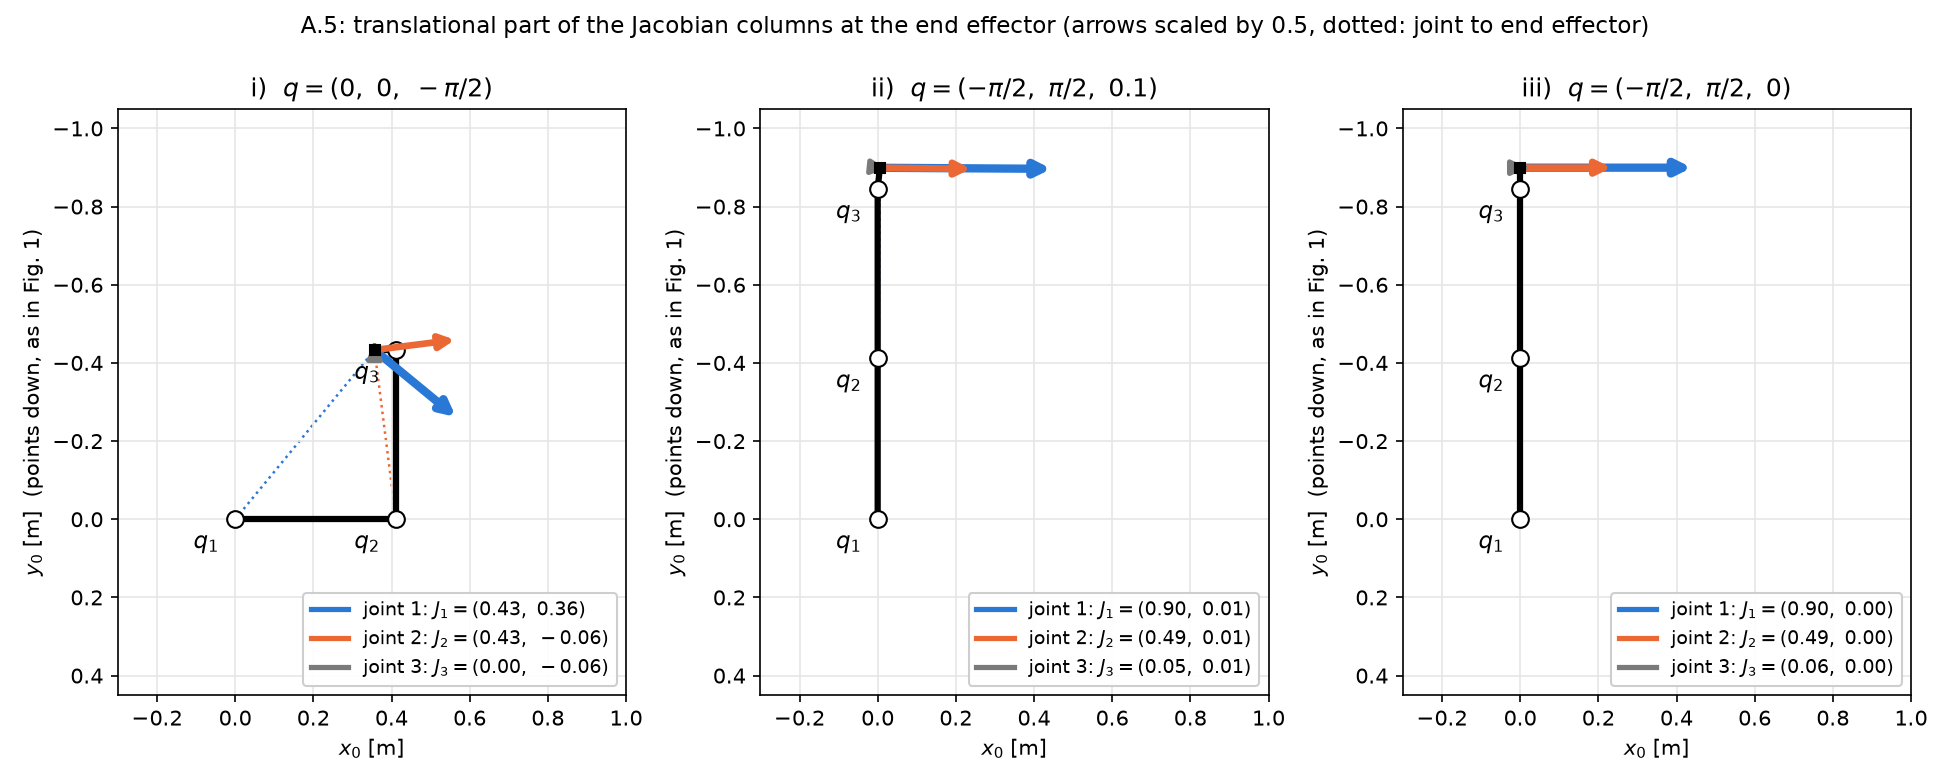
\includegraphics[width=0.72\textwidth]{a5_jacobian.png}
\end{center}
\vspace{-4pt}
\textbf{Pfeile zeichnen (Tutorial):} Linie vom Gelenk zur Hand (gepunktet). Der Pfeil steht senkrecht darauf, ist genauso
lang (im Plot halb so lang gezeichnet) und zeigt in Richtung einer positiven Drehung, also im Uhrzeigersinn. Die Zahlen sind
die $x$- und $y$-Einträge der Spalten von $J$.

\begin{itemize}
  \item \textbf{i: voll steuerbar.} Pfeil 1 und 2 zeigen in verschiedene Richtungen, zusammen erreicht man jede Richtung.
        Gelenk 3 dreht fast nur die Hand, damit stellt man die Orientierung.
  \item \textbf{ii: nahe an einer Singularität.} Arm fast gestreckt, alle Pfeile fast parallel (seitlich). Entlang des Arms
        nur $0.01$\,m/rad. Möglich, aber die Gelenke müssten dafür sehr schnell drehen.
  \item \textbf{iii: in einer Singularität.} Arm ganz gestreckt, alle Pfeile genau parallel. Entlang des Arms kann sich die
        Hand gar nicht bewegen, ein Freiheitsgrad fehlt.
\end{itemize}
\sagen{Verschiedene Richtungen = steuerbar, fast parallel = nahe an einer Singularität, genau parallel = Singularität.}

\begin{extra}
$\det J = -L_1 L_2\, c_2$ (Spalte 2 von Spalte 1 und Spalte 3 von Spalte 2 abziehen, dann entwickeln). In ii und iii ist
$q_2 = \frac{\pi}{2}$, also $\det J = 0$ in \emph{beiden}. Mit Orientierung gerechnet ist ii also schon singulär. Der
Grund: Glied 1 und 2 sind genau gestreckt. Die kleine Bewegung entlang des Arms in ii kommt nur von Gelenk 3, und das dreht
dabei immer auch die Hand, $\alpha$ ändert sich mit. Die Aufgabe fragt nach der Skizze (nur $x$, $y$), deshalb steht im
Bericht \glqq nahe\grqq. In i ist $q_2 = 0$, $\det J = -L_1 L_2 = -0.18 \ne 0$.
\end{extra}

\begin{fragen}
\frage{Woran erkennt man in der Skizze eine Singularität?}
{An den Richtungen der Pfeile. Zeigen alle in dieselbe Richtung (parallel), kann man aus ihnen keine Bewegung in die
andere Richtung zusammensetzen.}
\frage{Warum ist ii nur \glqq nahe\grqq{} und iii \glqq in\grqq{} der Singularität?}
{In ii haben die Pfeile wegen $q_3 = 0.1$ noch einen kleinen Anteil entlang des Arms ($0.01$\,m/rad), in iii ist er genau
null. In ii geht die Bewegung also noch, aber nur mit sehr großen Gelenkgeschwindigkeiten.}
\frage{Was passiert in der Nähe einer Singularität?}
{Eine kleine Bewegung im Arbeitsraum braucht eine riesige Bewegung im Gelenkraum (Tutorial T5). Das sieht man auch im
Bonus: Wo $|\det J|$ klein ist, wird der Fehler größer.}
\end{fragen}

%=====================================================================
\section{B1: Kubische Splines mit Via-Punkt}
%=====================================================================

Pro Gelenk zwei Splines: $q_a \to q_b$ ($0$--$2.5$\,s) und $q_b \to q_c$ ($2.5$--$5$\,s), $T = 2.5$\,s, Form aus dem Blatt
$q(t) = a_1 + a_2 (t - t_{start}) + a_3 (t - t_{start})^2 + a_4 (t - t_{start})^3$. Vier Bedingungen (Start- und Endwinkel,
Start- und Endgeschwindigkeit) für vier Parameter, Lösung aus dem Tutorial:
\[
  a_1 = q_s,\quad a_2 = \dot q_s,\quad
  a_3 = \frac{3}{T^2}(q_e - q_s) - \frac{2}{T}\dot q_s - \frac{1}{T}\dot q_e,\quad
  a_4 = -\frac{2}{T^3}(q_e - q_s) + \frac{1}{T^2}(\dot q_s + \dot q_e)
\]
\textbf{Annahme:} Start und Ende in Ruhe, $\dot q_a = \dot q_c = 0$. \textbf{Heuristik (Blatt, Craig):} Durchschnitts\-geschwindigkeiten
$v_1 = (q_b - q_a)/T = (-0.31,\ 0.63,\ 0)$, $v_2 = (q_c - q_b)/T = (-0.31,\ -0.31,\ 0)$ rad/s.
Gelenk 1: gleiches Vorzeichen $\Rightarrow$ Mittelwert $-0.31$. Gelenk 2: Vorzeichenwechsel $\Rightarrow$ 0. Gelenk 3:
bewegt sich nicht $\Rightarrow$ 0.

\begin{minipage}[c]{0.5\textwidth}
{\small
\begin{tabular}{ccrrrr}
  \toprule
  Gelenk & Segment & $a_1$ & $a_2$ & $a_3$ & $a_4$ \\
  \midrule
  1 & $a \to b$ & 0.00    & 0.00    & $-0.25$ & 0.05 \\
  1 & $b \to c$ & $-0.79$ & $-0.31$ & $-0.13$ & 0.05 \\
  2 & $a \to b$ & 0.00    & 0.00    & 0.75    & $-0.20$ \\
  2 & $b \to c$ & 1.57    & 0.00    & $-0.38$ & 0.10 \\
  3 & beide     & 0.00    & 0.00    & 0.00    & 0.00 \\
  \bottomrule
\end{tabular}
}
\end{minipage}\hfill
\begin{minipage}[c]{0.47\textwidth}
\textbf{Beispiel} Gelenk 1, erstes Segment:\\
$a_3 = \frac{3}{2.5^2}(-\frac{\pi}{4}) - \frac{-0.31}{2.5} = -0.38 + 0.13 = -0.25$\\
$a_4 = -\frac{2}{2.5^3}(-\frac{\pi}{4}) + \frac{-0.31}{2.5^2} = 0.10 - 0.05 = 0.05$\\
Im Plot: Kurven gehen durch $q_a, q_b, q_c$, kein Geschwindigkeitssprung am Via-Punkt.
\end{minipage}

\sagen{Zwei Splines pro Gelenk, die am Via-Punkt mit derselben Geschwindigkeit aneinanderhängen. Die Geschwindigkeit dort
kommt aus der Heuristik: Richtungswechsel 0, sonst Mittelwert.}

\begin{fragen}
\frage{Wann ist die Via-Geschwindigkeit null, wann der Mittelwert?}
{Pro Gelenk: Wechselt die Richtung (Gelenk 2 geht erst hoch, dann runter), ist sie 0. Sonst der Mittelwert der beiden
Durchschnittsgeschwindigkeiten (Gelenk 1). Gelenk 3 bewegt sich nicht, also 0.}
\frage{Warum kubisch und nicht linear?}
{Bei linearer Interpolation springt die Geschwindigkeit am Anfang und am Ende, das hieße unendliche Beschleunigung
(Tutorial). Mit kubischen Splines kann man die Geschwindigkeit an beiden Enden vorgeben, dadurch ist sie auch am Via-Punkt
stetig.}
\frage{Im Blatt heißen die Parameter $a_1 \ldots a_4$, im Code $a_0 \ldots a_3$?}
{Dasselbe, nur um eins verschoben. B1 nutzt die Schreibweise des Blatts, B2 die des \code{CubicSpline}-Structs.}
\end{fragen}

%=====================================================================
\section{B2: Spline im Gelenkraum (\code{njtrack}, \code{proj1})}
%=====================================================================

Beim Start rechnet \code{initNjtrackControl} einen Spline von \code{gv.q} nach \code{gv.qd}, Start und Ende in Ruhe.
Mit $\Delta q = q_d - q(t_0)$ (Tutorial):
$a_0 = q(t_0)$, $a_1 = 0$, $a_2 = \frac{3}{t_f^2}\Delta q$, $a_3 = -\frac{2}{t_f^3}\Delta q$.

\begin{herleitung}{\texorpdfstring{$t_f$}{tf} aus den Grenzen (wichtig)}
Ableiten ($t$ ab $t_0$):
\[
  \dot q_d(t) = 2a_2 t + 3a_3 t^2 = \frac{6\Delta q}{t_f^2}\,t - \frac{6\Delta q}{t_f^3}\,t^2, \qquad
  \ddot q_d(t) = 2a_2 + 6a_3 t = \frac{6\Delta q}{t_f^2} - \frac{12\Delta q}{t_f^3}\,t
\]
Die Geschwindigkeit ist eine \textbf{Parabel}, maximal in der Mitte $t = t_f/2$. Die Beschleunigung ist eine
\textbf{Gerade}, maximal am Anfang ($t = 0$) und am Ende:
\[
  |\dot q|_{\max} = \frac{3|\Delta q|}{2t_f} \le \dot q_{\max} \Rightarrow t_f \ge \frac{3|\Delta q|}{2\dot q_{\max}},
  \qquad
  |\ddot q|_{\max} = \frac{6|\Delta q|}{t_f^2} \le \ddot q_{\max} \Rightarrow t_f \ge \sqrt{\frac{6|\Delta q|}{\ddot q_{\max}}}
\]
$t_f$ = größter dieser Werte über alle Gelenke. proj1 aus der Nullstellung:

\centering
{\small
\begin{tabular}{lccc}
  \toprule
  & Gelenk 1 & Gelenk 2 & Gelenk 3 \\
  \midrule
  $|\Delta q|$ [rad] & 0.10 & 0.97 & 1.06 \\
  $t_f$ aus Geschwindigkeit [s] & 0.18 & 1.84 & 2.01 \\
  $t_f$ aus Beschleunigung [s] & 0.74 & 2.35 & \textbf{2.46} \\
  \bottomrule
\end{tabular}
}
\end{herleitung}

\secneed{11\baselineskip}
\begin{lstlisting}[firstnumber=41]
double computeTf(GlobalVariables& gv)
{
  double tf = 0.0;
  for (int i = 0; i < gv.dof; i++) {
    double distance = fabs(gv.qd[i] - gv.q[i]);
    double tf_velocity = 1.5 * distance / gv.dqmax[i];
    double tf_acceleration = sqrt(6.0 * distance / gv.ddqmax[i]);
    tf = max(tf, max(tf_velocity, tf_acceleration));
  }
  return tf;
}
\end{lstlisting}
\textbf{Z.\,41--51:} Pro Gelenk beide Grenzen aus der Herleitung, \code{1.5} $= \frac{3}{2}$. \code{max} merkt sich den
größten Wert. Grenzen aus \code{gv.dqmax} und \code{gv.ddqmax}, nicht hart codiert.

\secneed{10\baselineskip}
\begin{lstlisting}[firstnumber=58]
  spline.t0 = gv.curTime;
  spline.tf = computeTf(gv);

  PrVector distance = gv.qd - gv.q;
  spline.a0 = gv.q;
  spline.a1 = PrVector(gv.dof);
  if (spline.tf > 0.0) {
    spline.a2 = distance * (3.0 / (spline.tf * spline.tf));
    spline.a3 = distance * (-2.0 / (spline.tf * spline.tf * spline.tf));
\end{lstlisting}
\textbf{Z.\,24--31, 56--72:} \code{spline} ist global (Struct aus dem Blatt), damit die Init-Funktion ihn einmal rechnet
und der Regler ihn in jedem Takt benutzt. \code{PrVector(gv.dof)} ist ein Nullvektor ($a_1 = 0$). Der \code{else}-Zweig
(Z.\,67--71) setzt $a_2 = a_3 = 0$, damit es keine Division durch null gibt, wenn der Arm schon am Ziel steht. \code{initNjtrackControl} (Z.\,294--298) und
\code{initProj1Control} (Z.\,360--368) rufen \code{computeSpline} auf; proj1 setzt vorher \code{gv.qd} mit
\code{toRad(5.5)}, \code{toRad(55.4)}, \code{toRad(-60.8)} $= (0.096,\ 0.967,\ -1.061)$\,rad.

\secneed{13\baselineskip}
\begin{lstlisting}[firstnumber=78]
void followSpline(GlobalVariables& gv)
{
  double t = gv.curTime - spline.t0;
  if (t > spline.tf) {
    floatControl(gv);
    return;
  }

  gv.qd = spline.a0 + spline.a1 * t + spline.a2 * (t * t) + spline.a3 * (t * t * t);
  gv.dqd = spline.a1 + spline.a2 * (2.0 * t) + spline.a3 * (3.0 * t * t);

  gv.tau = -gv.kp * (gv.q - gv.qd) - gv.kv * (gv.dq - gv.dqd) + gv.G;
}
\end{lstlisting}
\textbf{Z.\,78--90:} Zeit seit dem Start, nach $t_f$ Float ($\tau = G$). Sonst Spline und seine Ableitung auswerten und
in \code{gv.qd}/\code{gv.dqd} schreiben, dann das Regelgesetz aus dem Blatt
$\tau = -k_p(q - q_d) - k_v(\dot q - \dot q_d) + G$. \code{*} zwischen \code{PrVector}s ist elementweise, jedes Gelenk hat
sein eigenes $k_p$. \code{njtrackControl} und \code{proj1Control} rufen nur \code{followSpline} auf.

\textbf{Ergebnis proj1:} $t_f = 2.46$\,s (Beschleunigungsgrenze von Gelenk 3). $q$ und $q_d$ liegen übereinander, Fehler
immer $< 0.01$\,rad, max.\ $55.5$\,Nm an Gelenk 1 (Grenze $156.4$). Gains $k_p = 3000/1350/300$, $k_v = 245/70/21$, von Hand
im Simulator getunt.

\sagen{Wir rechnen beim Start einen kubischen Spline pro Gelenk, alle mit derselben Dauer $t_f$. $t_f$ ist so gewählt, dass
kein Gelenk zu schnell wird oder zu stark beschleunigt. Ein PD-Regler mit Schwerkraftkompensation folgt dem Spline, danach
hält Float den Arm.}

\begin{fragen}
\frage{Woher kommen die zwei Grenzen für $t_f$?}
{Aus den Ableitungen des Splines. Die Geschwindigkeit ist eine Parabel mit Maximum bei $t_f/2$:
$\frac{3|\Delta q|}{2t_f}$. Die Beschleunigung ist eine Gerade mit Maximum bei $t = 0$: $\frac{6|\Delta q|}{t_f^2}$. Beides
$\le$ Grenze setzen und nach $t_f$ auflösen.}
\frage{Warum das Maximum über alle Gelenke? Warum kommen alle gleichzeitig an?}
{Jedes Gelenk muss seine Grenzen einhalten, also bestimmt das langsamste Gelenk die Dauer. Alle Splines haben dasselbe
$t_0$ und $t_f$ und sind bei $t_f$ genau am Ziel, deshalb kommen alle gleichzeitig an (verlangt in B2c). Die anderen Gelenke
bleiben dabei unter ihren Grenzen.}
\frage{Was passiert nach $t_f$?}
{Der Regler schaltet auf Float ($\tau = G$), wie im Blatt verlangt. Float hat keinen Positionsterm, deshalb bleibt ein
kleiner Fehler stehen.}
\frage{Warum dürfen die Gains viel höher sein als in A1?}
{In A1 sprang der Sollwert um $0.17$\,rad ($10^\circ$), der Fehler war am Anfang groß und damit auch das Drehmoment. Hier ändert sich
$q_d$ langsam und springt nicht, der Fehler bleibt klein. Deshalb bleibt auch $\tau$ mit großem $k_p$ unter der Grenze.}
\frage{Warum $\dot q - \dot q_d$ statt nur $\dot q$ wie in A1?}
{Das Blatt verlangt, auch die Soll-Geschwindigkeit zu verfolgen. Der Arm soll sich ja bewegen. Mit nur $-k_v\dot q$ würde der
D-Term die gewollte Bewegung bremsen, mit $\dot q - \dot q_d$ dämpft er nur die Abweichung.}
\end{fragen}

%=====================================================================
\section{C1: Kreis im Arbeitsraum (\code{proj2})}
%=====================================================================

\begin{herleitung}{Kreisbahn (wichtig)}
Position auf dem Kreis über den Winkel $\beta$, gemessen am Mittelpunkt $x_{c} = (0.6,\ 0.35)$\,m, ab dem Startpunkt.
Punkt auf dem Kreis = Mittelpunkt + $r\,(\cos\beta, \sin\beta)$, $r = 0.2$\,m, Orientierung bleibt 0:
\[
  x_d = \begin{pmatrix} 0.6 + r\cos\beta \\ 0.35 + r\sin\beta \\ 0 \end{pmatrix},
  \qquad \beta(t) = \dot\beta\,(t - t_{start}),\quad \dot\beta = \frac{2\pi}{5}\,\text{rad/s}
\]
Der Regler braucht auch die Soll-Geschwindigkeit, also $x_d$ nach der Zeit ableiten (Kettenregel, $\frac{d}{dt}\cos\beta =
-\dot\beta\sin\beta$):
\[
  \dot x_d = \begin{pmatrix} -r\,\dot\beta\sin\beta \\ r\,\dot\beta\cos\beta \\ 0 \end{pmatrix}
\]
Checks: $\beta = 0$ gibt $(0.8,\ 0.35)$ = Startpunkt aus dem Blatt. Eine Runde dauert $2\pi/\dot\beta = 5$\,s.
Bahngeschwindigkeit $r\dot\beta = 0.2 \cdot 1.26 = 0.25$\,m/s.
\end{herleitung}

\secneed{10\baselineskip}
\begin{lstlisting}[firstnumber=119]
void setCircleTarget(GlobalVariables& gv, double beta, double dbeta)
{
  gv.xd[0] = CIRCLE_CENTER_X + CIRCLE_RADIUS * cos(beta);
  gv.xd[1] = CIRCLE_CENTER_Y + CIRCLE_RADIUS * sin(beta);
  gv.xd[2] = 0.0;

  gv.dxd[0] = -CIRCLE_RADIUS * dbeta * sin(beta);
  gv.dxd[1] = CIRCLE_RADIUS * dbeta * cos(beta);
  gv.dxd[2] = 0.0;
}
\end{lstlisting}
\vspace{-4pt}
\secneed{8\baselineskip}
\begin{lstlisting}[firstnumber=510]
void proj2Control(GlobalVariables& gv)
{
  // constant angular velocity: beta grows linearly with time
  double beta = CIRCLE_ANGULAR_VELOCITY * (gv.curTime - circle_start_time);
  setCircleTarget(gv, beta, CIRCLE_ANGULAR_VELOCITY);
  operationalSpaceControl(gv);
}
\end{lstlisting}
\textbf{Z.\,96--112:} Konstanten (\code{PI}, Mittelpunkt, Radius, $\dot\beta = 2\pi/5$) und \code{circle\_start\_time}.
\textbf{Z.\,119--128:} genau die Formeln aus der Herleitung. Wir haben sie in eine Funktion gelegt, weil proj3 und der Bonus
denselben Kreis brauchen, nur mit anderem $\beta(t)$. \textbf{Z.\,370--374:} \code{initProj2Control} merkt sich die
Startzeit. \textbf{Z.\,510--516:} $\beta$ wächst linear mit der Zeit.

\sagen{Wir beschreiben den Kreis über einen Winkel $\beta$, der linear mit der Zeit wächst. Daraus folgen Soll-Position und,
durch Ableiten, Soll-Geschwindigkeit.}

\begin{fragen}
\frage{In welche Richtung läuft der Kreis?}
{Positives $\beta$ dreht um die $z$-Achse des Simulators, $z$ zeigt aus dem Bildschirm heraus. Auf dem Bildschirm also
\textbf{gegen den Uhrzeigersinn}, vom Startpunkt rechts erst nach oben (wie der Pfeil in Fig.~3). Schaut man in die positive
$z$-Richtung, ist es im Uhrzeigersinn, so steht es im Blatt.}
\frage{Warum gebt ihr auch $\dot x_d$ vor?}
{Der Regler hat einen D-Term auf $\dot x - \dot x_d$. Ohne $\dot x_d$ würde er die Bewegung entlang des Kreises bremsen.}
\frage{Wie kommt der Arm zum Startpunkt?}
{Mit \code{proj1}. Dessen Zielwinkel liegen genau am Kreisstart (beobachtet: $x \approx (0.80,\ 0.35,\ 0)$ nach proj1). Die
Aufnahme haben wir erst danach gestartet, wie im Blatt verlangt.}
\end{fragen}

%=====================================================================
\section{C2: Regelung im Arbeitsraum}
%=====================================================================

\[
  F = -k_p\,(x - x_d) - k_v\,(\dot x - \dot x_d), \qquad \tau = J^T(q)\,F + G(q)
\]
Erst eine Kraft am Endeffektor (Feder und Dämpfer zwischen $x$ und $x_d$), die dritte Komponente ist ein Moment für die
Orientierung. Dann mit der transponierten Jacobi-Matrix in Gelenkmomente umrechnen und die Schwerkraft dazu (Vorlesung).

\secneed{6\baselineskip}
\begin{lstlisting}[firstnumber=136]
void operationalSpaceControl(GlobalVariables& gv)
{
  PrVector F = -gv.kp * (gv.x - gv.xd) - gv.kv * (gv.dx - gv.dxd);
  gv.tau = gv.Jtranspose * F + gv.G;
}
\end{lstlisting}
\textbf{Z.\,136--140:} Alles vom Simulator: \code{gv.x} $= (x, y, \alpha)$, \code{gv.dx}, \code{gv.Jtranspose}
($3 \times 3$), \code{gv.G}. Hier ist \code{*} ein Matrix-mal-Vektor-Produkt. Im Blatt steht \code{gv.Jtransposed}, im
Header heißt es \code{gv.Jtranspose}.

\sagen{Wir rechnen den Fehler direkt in $x$, $y$, $\alpha$, machen daraus eine Federkraft an der Hand und verteilen sie mit
$J^T$ auf die Gelenke. So brauchen wir nie die Gelenkwinkel zum Kreis, also keine inverse Kinematik.}

\begin{fragen}
\frage{Warum braucht ihr keine inverse Kinematik?}
{Wir brauchen nie $q_d$. Der Fehler wird im Arbeitsraum gerechnet und über $J^T$ direkt in Drehmomente umgerechnet. Das
Blatt sagt selbst, dass man damit die inverse Kinematik umgeht.}
\frage{Was macht $J^T$?}
{Es rechnet eine Kraft (und ein Moment) an der Hand in Gelenkmomente um. Zeile $j$ von $J^T$ ist Spalte $j$ von $J$, also
die Richtung, in die Gelenk $j$ die Hand bewegt. Jedes Gelenk bekommt den Anteil der Kraft, der in seine
Bewegungsrichtung zeigt.}
\frage{Warum die Jacobi-Matrix des Simulators und nicht eure aus Teil A?}
{Das Blatt verlangt es, sie ist im Simulatorframe (wie \code{gv.x}), und wir dürfen nur \code{control.cpp} abgeben. Unsere
aus Teil A ist im Frame von Fig.~1.}
\end{fragen}

%=====================================================================
\secneed{16\baselineskip}
\section{C3: Gain-Tuning und Fehler über \texorpdfstring{$k_p$}{kp}}
%=====================================================================

\begin{minipage}[c]{0.36\textwidth}
\centering
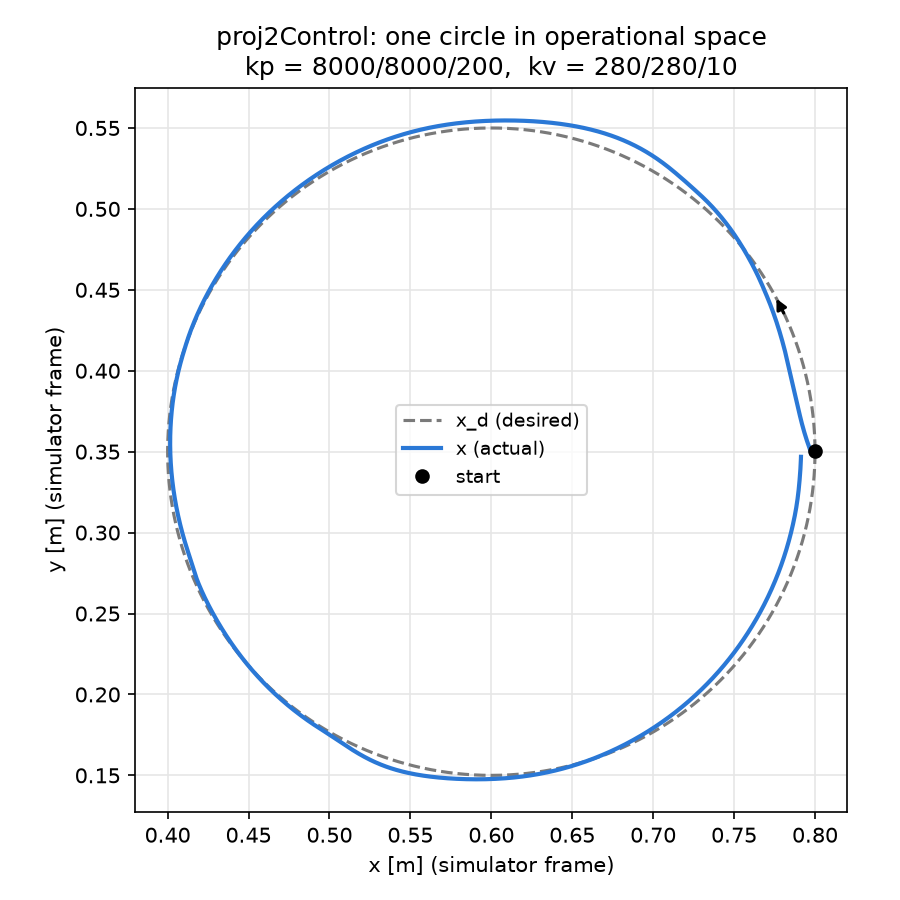
\includegraphics[width=\textwidth]{proj2_xy.png}
\end{minipage}\hfill
\begin{minipage}[c]{0.61\textwidth}
\textbf{Gains:} $k_p = 8000/8000/200$, $k_v = 280/280/10$ für $(x, y, \alpha)$.

\textbf{Ergebnis:} Positionsfehler immer $< 11$\,mm, Orientierung $< 0.03$\,rad. Spitzen $116 / 38 / 1$\,Nm (Grenzen
$156.4 / 89.4 / 20.1$).

\textbf{Spitze am Anfang:} Der Arm steht, aber $\dot x_d$ springt von 0 auf $r\dot\beta = 0.25$\,m/s. Der D-Term will sofort
eine große Kraft. Im $x$-$y$-Plot verlässt die Hand kurz nach dem Start den Kreis.

\smallskip
{\small
\begin{tabular}{lccccc}
  \toprule
  $k_p$ ($x$, $y$) & 1000 & 2000 & 4000 & 8000 & 12000 \\
  \midrule
  RMS-Fehler [mm] & 47 & 26 & 14 & 7 & 5 \\
  \bottomrule
\end{tabular}
}
\end{minipage}

\textbf{Fehler $\sim 1/k_p$:} Doppeltes $k_p$, halber Fehler, die Form der Kurve bleibt gleich. Unsere Erklärung: Der Regler
ist eine Feder zwischen $x$ und $x_d$. Für die Bewegung auf dem Kreis braucht der Arm eine bestimmte Kraft, und eine Feder
mit Steifigkeit $k_p$ muss dafür um $e = F/k_p$ gedehnt werden.

\textbf{Grenzen:} $k_p = 12000$ gibt 5\,mm, aber $146$\,Nm an Gelenk 1, zu knapp an $156.4$. $k_v$ haben wir mit $k_p$
erhöht, damit nichts schwingt. Viel größeres $k_v$ geht auch nicht: $k_v = 500$ gibt durch den Geschwindigkeitssprung
$168$\,Nm.

\sagen{Je steifer die Feder $k_p$, desto kleiner der Fehler, ungefähr $\propto 1/k_p$. Die Grenze ist das Drehmoment an
Gelenk 1.}

\begin{fragen}
\frage{Wie ändert sich der Fehler mit $k_p$?}
{Ungefähr $\propto 1/k_p$: $47 \to 26 \to 14 \to 7$\,mm bei $1000 \to 8000$. Die Form bleibt, die Kurve wird nur kleiner.}
\frage{Was begrenzt $k_p$ und $k_v$?}
{Die Drehmomentgrenzen, vor allem an Gelenk 1 (siehe oben). Zu kleines $k_v$ lässt die Hand schwingen.}
\frage{Warum ist die größte Spitze genau am Start?}
{Die Soll-Geschwindigkeit springt von 0 auf 0.25\,m/s, der Arm steht noch. Der D-Term sieht einen großen Fehler
$\dot x - \dot x_d$ und erzeugt eine große Kraft. Das behebt C4.}
\end{fragen}

%=====================================================================
\section{C4: Parabolic Blends (\code{proj3})}
%=====================================================================

\begin{herleitung}{Parabolic Blends für \texorpdfstring{$\beta$}{beta} (wichtig)}
Drei Teile: Blend mit konstanter Beschleunigung $\ddot\beta = \frac{2\pi}{25}$, linearer Teil mit $\dot\beta = \frac{2\pi}{5}$,
Blend mit konstanter Verzögerung bis 0.

\textbf{Blendzeit} (Hinweis im Blatt): $\dot\beta(t_b) = t_b\,\ddot\beta = \frac{2\pi}{5}
\;\Rightarrow\; t_b = \frac{\dot\beta}{\ddot\beta} = \frac{2\pi/5}{2\pi/25} = 5$\,s.

\textbf{Gesamtzeit:} Winkel in einem Blend $\frac12\ddot\beta\,t_b^2 = \frac12 \cdot \frac{2\pi}{25} \cdot 25 = \pi$. Drei
Runden sind $\beta_f = 6\pi$. Beide Blends zusammen $2\pi$, bleiben $4\pi$ für den linearen Teil, das dauert
$4\pi / \frac{2\pi}{5} = 10$\,s. Also $t_f = 5 + 10 + 5 = 20$\,s.
\[
  \beta(t) =
  \begin{cases}
    \frac12\ddot\beta\,t^2 & 0 \le t < t_b \\[2pt]
    \frac12\ddot\beta\,t_b^2 + \dot\beta\,(t - t_b) & t_b \le t < t_f - t_b \\[2pt]
    \beta_f - \frac12\ddot\beta\,(t_f - t)^2 & t_f - t_b \le t < t_f \\[2pt]
    \beta_f & t \ge t_f
  \end{cases}
  \qquad
  \dot\beta(t) =
  \begin{cases}
    \ddot\beta\,t \\[2pt]
    \dot\beta \\[2pt]
    \ddot\beta\,(t_f - t) \\[2pt]
    0
  \end{cases}
\]
Der zweite Blend ist der erste gespiegelt, rückwärts vom Ende gezählt. Übergänge stetig: bei $t_b$ ist $\beta = \pi$, bei
$t_f - t_b = 15$\,s ist $\beta = \pi + 4\pi = 6\pi - \pi = 5\pi$, die Geschwindigkeit passt jeweils auch.
$\beta$ und $\dot\beta$ gehen in \code{setCircleTarget} aus C1, Regler wie in C2.
\end{herleitung}

\begin{minipage}[t]{0.66\textwidth}
\vspace{0pt}
\begin{lstlisting}[firstnumber=531]
  double t = gv.curTime - circle_start_time;
  double acc = CIRCLE_ANGULAR_ACCELERATION;
  double vel = CIRCLE_ANGULAR_VELOCITY;
  double tb = vel / acc;
  double tf = CIRCLE_TOTAL_ANGLE / vel + tb;

  double beta, dbeta;
  if (t < tb) {
    beta = 0.5 * acc * t * t;
    dbeta = acc * t;
  } else if (t < tf - tb) {
    beta = 0.5 * acc * tb * tb + vel * (t - tb);
    dbeta = vel;
  } else if (t < tf) {
    // mirror image of blend 1, measured backwards from the end
    double t_left = tf - t;
    beta = CIRCLE_TOTAL_ANGLE - 0.5 * acc * t_left * t_left;
    dbeta = acc * t_left;
  } else {
    beta = CIRCLE_TOTAL_ANGLE;
    dbeta = 0.0;
  }

  setCircleTarget(gv, beta, dbeta);
  operationalSpaceControl(gv);
\end{lstlisting}
\end{minipage}\hfill
\begin{minipage}[t]{0.32\textwidth}
\vspace{0pt}
\centering
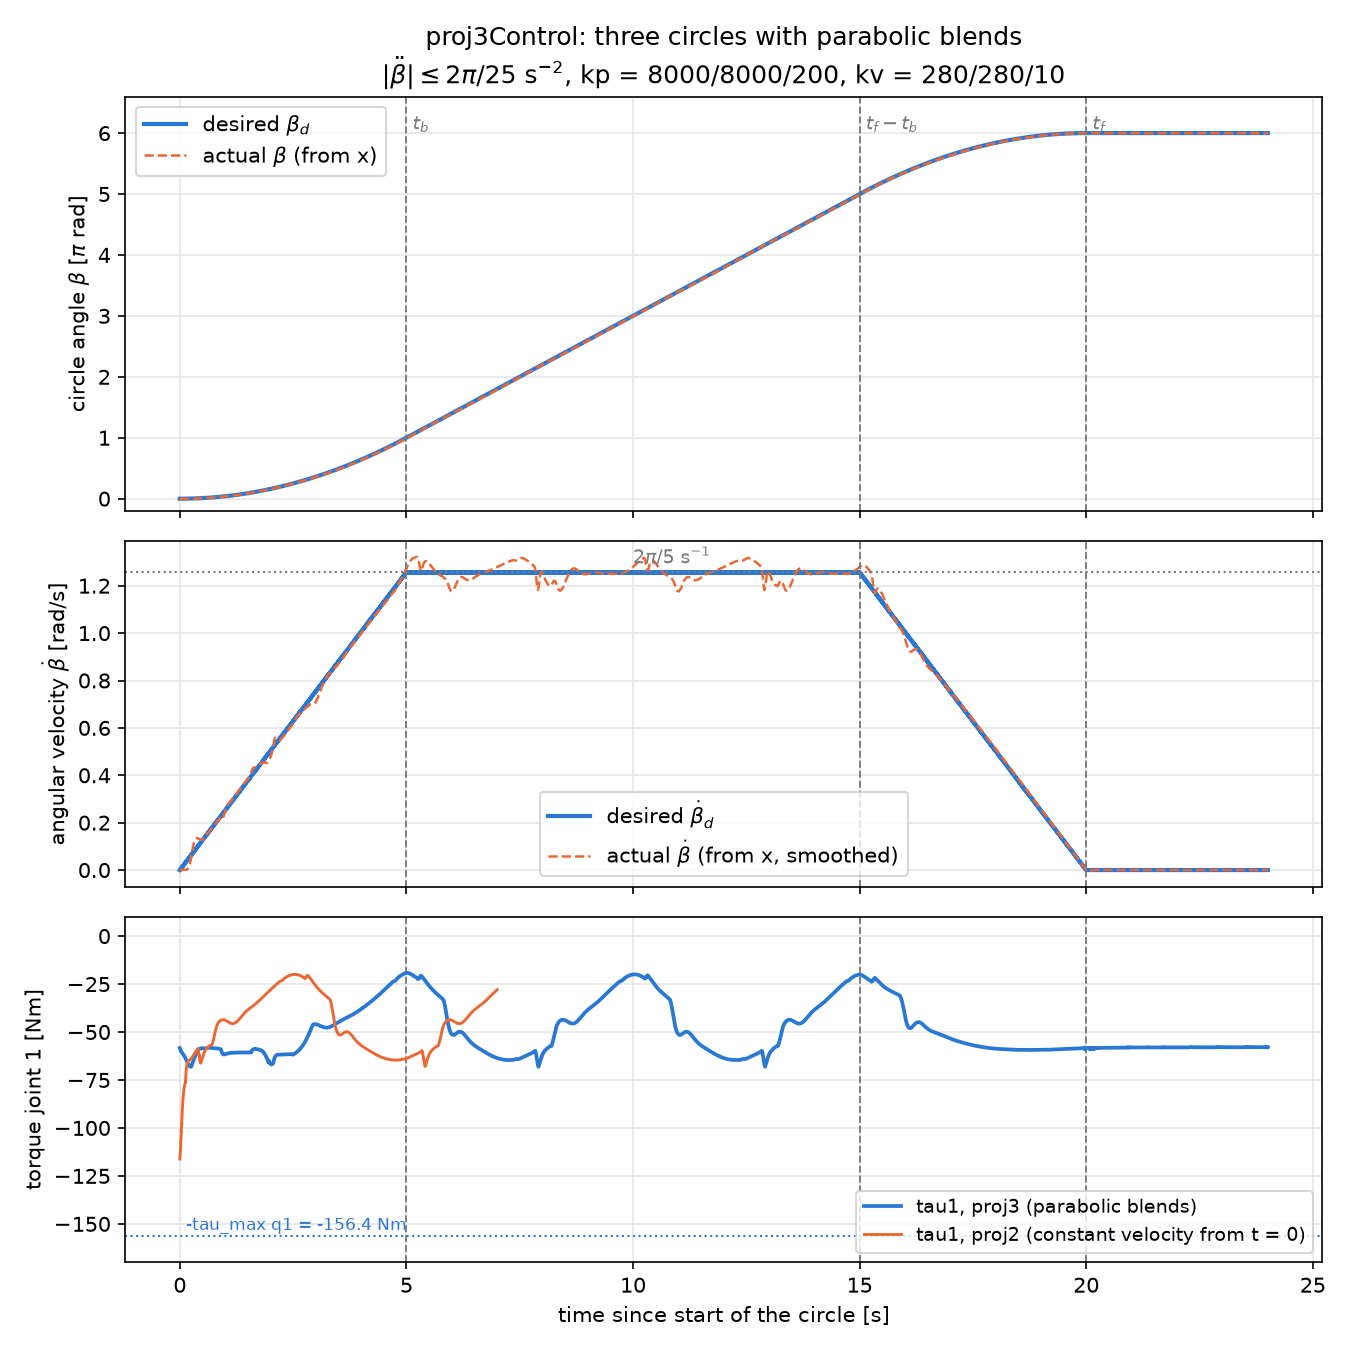
\includegraphics[width=\textwidth]{proj3_blends.png}
\end{minipage}

\textbf{Z.\,108--109:} $\ddot\beta = 2\pi/25$, $\beta_f = 3 \cdot 2\pi$. \textbf{Z.\,534--535:} $t_b$ und $t_f$ werden
gerechnet, nicht eingetippt. $t_f = \beta_f/\dot\beta + t_b = 15 + 5 = 20$\,s ist dasselbe wie $2t_b + 4\pi/\dot\beta$, weil
$2 \cdot \frac12\ddot\beta t_b^2 / \dot\beta = t_b$. \textbf{Z.\,538--552:} die vier Fälle der Formel.

\textbf{Ergebnis:} gleiche Gains wie proj2. Fehler wieder $< 11$\,mm, keine Spitze am Start mehr: max.\ $68$\,Nm an Gelenk 1
statt $116$\,Nm bei proj2. Nach 20\,s ($\beta = 6\pi$, $\dot\beta = 0$) hält die Hand den Endpunkt, das ist wieder der
Startpunkt $(0.8,\ 0.35)$.

\sagen{Statt sofort mit voller Geschwindigkeit loszufahren, beschleunigt $\beta$ 5\,s lang gleichmäßig, fährt 10\,s konstant
und bremst 5\,s. So springt die Soll-Geschwindigkeit nie, und die Drehmomentspitze am Start ist weg.}

\begin{fragen}
\frage{Warum Parabolic Blends?}
{In proj2 springt die Soll-Geschwindigkeit beim Start (und beim Stoppen). Mit begrenzter Beschleunigung steigt sie linear an,
es gibt keinen Sprung und keine Drehmomentspitze mehr.}
\frage{Wie kommt ihr auf $t_b$ und $t_f$?}
{$t_b$: Am Ende des Blends muss die Geschwindigkeit $\frac{2\pi}{5}$ sein, also $t_b \cdot \frac{2\pi}{25} = \frac{2\pi}{5}$,
$t_b = 5$\,s. $t_f$: Jeder Blend schafft $\pi$, für den linearen Teil bleiben $4\pi$, das sind $10$\,s, zusammen $20$\,s.}
\frage{Wird die Beschleunigungsgrenze eingehalten?}
{Ja. In den Blends ist $|\ddot\beta| = \frac{2\pi}{25}$ genau an der Grenze, im linearen Teil ist sie 0.}
\end{fragen}

%=====================================================================
\section{C5: Bonus}
%=====================================================================

Für den Bonus haben wir Regler der Vorlage benutzt, die sonst frei waren, so bleibt alles in \code{control.cpp}. Alle mit
dem Regler aus C2, den Gains von proj2 und derselben Bahngeschwindigkeit $0.25$\,m/s, Start am Kreisstart.

\begin{minipage}[c]{0.5\textwidth}
\begin{itemize}
  \item \code{lineControl}: Linie $(0.8, 0.35) \leftrightarrow (0.4, 0.35)$, hin und zurück.
  \item \code{xtrackControl}: Quadrat, Seite $0.2$\,m, gegen den Uhrzeigersinn wie der Kreis.
  \item \code{nxtrackControl}: Kreis + Rauschen, pro Takt zufällig $\pm 10\,\%$ von $\tau_{\max}$.
  \item \code{ntrackControl}: Kreis, aber nur $80\,\%$ von $G$.
\end{itemize}
\end{minipage}\hfill
\begin{minipage}[c]{0.47\textwidth}
\centering
{\small
\begin{tabular}{lccc}
  \toprule
  Bahn & max. & RMS & max.\ $|\tau_1|$ \\
  \midrule
  Kreis & 11\,mm & 7\,mm & 116\,Nm \\
  Linie & 22\,mm & 9\,mm & 99\,Nm \\
  Quadrat & 50\,mm & 19\,mm & 138\,Nm \\
  \bottomrule
\end{tabular}
}
\end{minipage}

\secneed{8\baselineskip}
\begin{lstlisting}[firstnumber=445]
void nxtrackControl(GlobalVariables& gv)
{
  bonusCircle(gv);
  for (int i = 0; i < gv.dof; i++) {
    gv.tau[i] += NOISE_RATIO * gv.taumax[i] * randomUnit();
  }
}
\end{lstlisting}
\textbf{Z.\,445--451:} erst der normale Kreis (\code{bonusCircle}, Z.\,225--230), dann auf jedes Moment eine Zufallszahl
zwischen $-10\,\%$ und $+10\,\%$ von $\tau_{\max}$. \code{randomUnit} (Z.\,218--222) ist ein einfacher eigener
Zufallsgenerator, damit kein weiteres Include nötig ist; der feste Startwert gibt in jedem Lauf dasselbe Rauschen.
\textbf{Z.\,482--486:} \code{ntrackControl} rechnet ebenfalls erst den normalen Kreis und zieht dann
\code{gv.G * (1.0 - GRAVITY\_COMPENSATION\_RATIO)} ab, also $\tau = J^T F + G - 0.2\,G = J^T F + 0.8\,G$.

\textbf{Ergebnisse (gegenüber dem normalen Kreis):}
\begin{itemize}
  \item \textbf{Rauschen:} im Mittel nur $0.7$\,mm (max.\ $1.9$\,mm), obwohl bis $15.6$\,Nm an Gelenk 1. Das Rauschen ist in
        jedem Takt anders und im Mittel null. Der schwere Arm folgt so schnellen Änderungen nicht, den Rest korrigiert der
        Regler.
  \item \textbf{80\,\% von $G$:} im Mittel $2.6$\,mm (max.\ $3.9$\,mm). Das fehlende Moment ist immer da und wirkt immer in
        dieselbe Richtung. Der P-Term muss es ersetzen und braucht dafür einen Fehler.
  \item \textbf{Nicht überall gleich:} Mit dem $G$-Fehler schwankt die Abweichung entlang des Kreises zwischen $1.7$ und
        $3.9$\,mm. Groß ist sie, wo $|\det J|$ klein ist ($0.10$--$0.12$, näher an einer Singularität), klein, wo $|\det J|$
        groß ist ($0.16$--$0.18$). Unsere Erklärung: Über $\tau = J^T F$ braucht der Regler nahe einer Singularität eine
        größere Kraft für dasselbe Moment, und größere Kraft heißt größerer Fehler. Außerdem hängt das fehlende Moment selbst
        von der Stellung ab.
\end{itemize}

\sagen{Glatte Bahnen sind leicht, Sprünge in der Geschwindigkeit sind schwer. Rauschen mittelt sich weg, ein konstanter
Modellfehler nicht, und wie stark er wirkt, hängt von der Stellung ab.}

\begin{fragen}
\frage{Welche Bahnen sind leicht, welche schwer, und warum?}
{Leicht: glatte Bahnen wie der Kreis, die Geschwindigkeit ändert ihre Richtung langsam. Schwer: Sprünge in der
Geschwindigkeit, also die Wendepunkte der Linie ($-0.25 \to +0.25$\,m/s) und die Ecken des Quadrats (Vierteldrehung). Dafür
bräuchte man unendliche Beschleunigung, der Arm schießt über, und der D-Term gibt eine Spitze. Auf den geraden Stücken sind
Linie und Quadrat so gut wie der Kreis. Derselbe Effekt wie proj2 gegen proj3.}
\frage{Warum stört Rauschen weniger als ein konstanter Fehler?}
{Rauschen ist im Mittel null und wechselt jeden Takt, der Arm mittelt es weg. Ein konstanter Fehler in $G$ zieht immer in
dieselbe Richtung, das muss der P-Term mit einem bleibenden Fehler ausgleichen.}
\frage{Ist das Verhalten im ganzen Arbeitsraum gleich?}
{Nein. Die Abweichung hängt von der Stellung ab: größer, wo $|\det J|$ klein ist, also näher an einer Singularität.}
\end{fragen}

%=====================================================================
\section{Allgemeine Fragen (jeder muss sie beantworten können)}
%=====================================================================

\begin{fragen}
\frage{Warum C++98, kein \code{new}, nur statischer Speicher?}
{Steht in den Coding-Regeln: Der Code soll auch auf dem echten Puma laufen, auf einem Echtzeit-PC mit QNX und 500\,Hz
Regeltakt. Deshalb z.\,B.\ die globale Variable \code{spline} statt dynamischem Speicher.}
\frage{Warum keine Ausgaben (\code{printf}/\code{cout})?}
{Ausgaben dauern zu lange und würden den Regeltakt stören. \code{PrintDebug} der Vorlage bleibt unverändert, es läuft nur
auf den Befehl \code{pdebug}.}
\frage{Wo stehen die Gains?}
{Nie im Code, immer \code{gv.kp}/\code{gv.kv}. Gespeichert mit \glqq Store gains\grqq{} in \code{gains\_1.txt} (\code{\_1} =
3-DOF-Modus), pro Regler ein Block: Anzahl Gelenke, $k_p$-Zeile, $k_v$-Zeile.}
\frage{Begrenzt ihr das Drehmoment im Code?}
{Nein, das verbietet das Blatt. Wir haben mit ausgeschalteten \glqq torque limits\grqq{} getestet und die Gains so gewählt,
dass die Spitzen unter $\tau_{\max}$ bleiben (proj1 $55.5$, proj2 $116$, proj3 $68$\,Nm an Gelenk 1).}
\frage{Gelenkraum oder Arbeitsraum -- Vor- und Nachteile?}
{Gelenkraum (Teil B): einfach, keine Probleme mit Singularitäten, aber die Hand fährt keine vorgegebene Form. Arbeitsraum
(Teil C): man kann Formen wie einen Kreis fahren, aber es gibt Probleme nahe Singularitäten (Tutorial T5).}
\frage{Woher kommt $G$ in A2?}
{Aus dem Simulator (\code{gv.G}), wie im Blatt verlangt. \code{PreprocessControl} rechnet unser Modell aus A1 nicht mehr.}
\end{fragen}

\end{document}
